\section*{Esercizi del 2 maggio}

\subsection*{Esercizio 4.2}
A meno di restringere $\nu K$, operazione che preserva il tipo di omotopia di $M$, possiamo supporre che la chiusura di $\nu K$ sia contenuta nella parte interna di un intorno tubolare compatto $D^2\times S^1\subs S^3$ di $K$.

\begin{itemize}
\item Consideriamo gli aperti $U=\interior M$, $V=\interior (D^2\times S^1)$ di $S^3$. Osserviamo che $U$ è omotopicamente equivalente a $M$, $V$ è omotopicamente equivalente a $S^1$, e $U\cap V$ è omotopicamente equivalente a $T^2$. Scriviamo una parte della successione esatta di Mayer-Vietoris relativa a $U$ e $V$:
\begin{diagram}
H_2(S^3)\rar&H_1(T^2)\rar&H_1(S^1)\dirsum H_1(M)\rar&H_1(S^3),
\end{diagram}
da cui
\begin{diagram}
0\rar&\ZZ\dirsum\ZZ\rar&\ZZ\dirsum H_1(M)\rar&0.
\end{diagram}
Poiché $H_1(M)$ è abeliano e finitamente generato ($M$ è compatta), segue immediatamente che $H_1(M)\iso\ZZ$.
\item Mostriamo che l'omomorfismo $H_1(T^2)\to H_1(M)$ indotto dall'inclusione è suriettivo.
\begin{itemize}
\item\textbf{Vale $H_1(S^3,\overline{\nu K})=0$.} Infatti dalla successione esatta lunga in omologia relativa per la coppia $(S^3,\overline{\nu K})$ otteniamo
\begin{diagram}
H_1(S^3)\rar&H_1(S^3,\overline{\nu K})\rar&\widetilde{H}_0(\overline{\nu K}),
\end{diagram}
da cui (osservando che $H_1(S^3)=\widetilde{H}_0(\overline{\nu K})=0$) la tesi.
\item\textbf{Vale $H_1(M,T^2)=0$.} Poiché $M=S^3\setminus\nu K$ e $T^2=\overline{\nu K}\setminus\nu K$, per escissione otteniamo
\[
H_1(M,T^2)=H_1(S^3\setminus\nu K,\overline{\nu K}\setminus\nu K)\iso H_1(S^3,\overline{\nu K})=0.
\]
\item\textbf{L'omomorfismo $H_1(T^2)\to H_1(M)$ è suriettivo.} Infatti dalla successione esatta lunga della coppia $(M,T^2)$ otteniamo
\begin{diagram}
H_1(T^2)\rar&H_1(M)\rar&H_1(M,T^2)=0.
\end{diagram}
\end{itemize}
Ma allora il nucleo di questo omomorfismo è un sottogruppo ciclico di $H_1(T^2)\iso\ZZ\dirsum\ZZ$ generato da un elemento primitivo, diciamo $\alpha\in H_1(T^2)$. Sappiamo che tale $\alpha$ è rappresentato (a meno dell'orientazione) da un'unica classe di isotopia di curve semplici chiuse, il che permette di definire la \defterm{longitudine}.
\item Si vede facilmente che l'omomorfismo $H_1(T_2)\to H_1(D^2\times S^1)$ è suriettivo, poiché ogni curva chiusa in $D^2\times S^1$ che rappresenta un generatore di $H_1(D^2\times S^1)$ è omotopa a una curva con supporto contenuto in $T_2$. Allora, esattamente come nel punto precedente, il nucleo di tale omomorfismo è generato da un elemento primitivo di $H_1(T^2)$, al quale corrisponde (a meno dell'orientazione) un'unica classe di isotopia di curve semplici chiuse. Questo permette di definire il \defterm{meridiano}.
\end{itemize}

\newpage
\subsection*{Esercizio 4.3}
\tikzfading[name=fade out,inner color=transparent!0,outer color=transparent!100]
\tikzset{
pics/tetrahedron/.style={
code={
\coordinate (#1-1) at (0,0);
\coordinate (#1-2) at (1.8,-.7);
\coordinate (#1-3) at (2.5,.4);
\coordinate (#1-4) at (1,1.8);
}},
on each segment/.style={
decorate,
decoration={
show path construction,
lineto code={\path [#1] (\tikzinputsegmentfirst) -- (\tikzinputsegmentlast);},
closepath code={\path [#1] (\tikzinputsegmentfirst) -- (\tikzinputsegmentlast);}
}},
mid arrow/.style={postaction={decorate,decoration={
markings,
mark=at position .5 with {\arrow[scale=1.5,#1]{latex}}
}}},
}
Ricordiamo che una struttura iperbolica sul complementare del nodo figura otto è data dall'incollamento secondo il seguente schema di due tetraedri ideali regolari iperbolici aventi orientazione opposta (le facce dello stesso colore vengono identificate, in modo da rispettare le orientazioni e i colori rappresentati sugli spigoli).

\begin{center}
\begin{tikzpicture}
\pic[scale=1.5] at (0,0) {tetrahedron=a};
\pic[scale=1.5] at (6,0) {tetrahedron=b};
\foreach \T in {a,b} {
\begin{scope}[on background layer={opacity=.4}]
\fill[orange] (\T-1) -- (\T-2) -- (\T-3) -- cycle;
\fill[green] (\T-1) -- (\T-3) -- (\T-4) -- cycle;
\end{scope}
\begin{scope}[opacity=.3]
\fill[white] (\T-1) -- (\T-2) -- (\T-4) -- cycle;
\fill[black] (\T-2) -- (\T-3) -- (\T-4) -- cycle;
\end{scope}
}
\draw[blue,thick,postaction={on each segment={mid arrow}}] (a-1) -- (a-2) (a-3) -- (a-2) (a-3) -- (a-4) (b-2) -- (b-3) (b-2) -- (b-4);
\draw[red,thick,postaction={on each segment={mid arrow}}] (a-1) -- (a-4) (a-2) -- (a-4) (b-2) -- (b-1) (b-4) -- (b-1) (b-4) -- (b-3);
\begin{scope}[on background layer={thick,opacity=.7,dashed}]
\draw[blue,postaction={mid arrow}] (b-1) -- (b-3);
\draw[red,postaction={mid arrow}] (a-1) -- (a-3);
\end{scope}
\foreach \T in {a,b} {
\foreach \i/\pos in {1/east,2/north,3/west,4/south} {
\draw[fill=white] (\T-\i) circle (2pt);
\node[inner sep=5pt,anchor=\pos] at (\T-\i) {$\T_{\i}$};
}}
\node[anchor=east] at ($(a-4)+(-1.5,-.5)$) {$T\times\{0\}$};
\node[anchor=west] at ($(b-4)+(2,-.5)$) {$T\times\{1\}$};
\end{tikzpicture}
\end{center}

Per fissare la notazione, siano $M$ il complementare del nodo figura otto, $T\times\{0,1\}$ l'unione disgiunta dei due tetraedri $T\times\{0\}$ e $T\times\{1\}$, $\sim$ la relazione di equivalenza descritta dall'incollamento, in modo che $M=T\times\{0,1\}/\sim$. Ricordiamo che, essendo $T$ un tetraedro ideale regolare iperbolico, ogni permutazione dei suoi vertici è indotta da un'isometria di $\HH^3$. Sia allora $\map{g}{T}{T}$ l'isometria di $T$ che induce la permutazione $\sigma=(1\;2)(3\;4)$.
\begin{center}
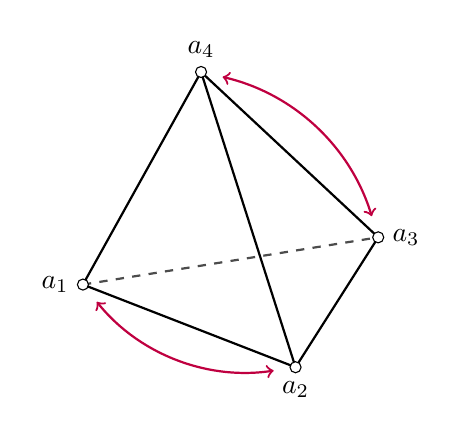
\begin{tikzpicture}
\pic[scale=1.5] {tetrahedron=a};
\draw[thick,opacity=.7,dashed] (a-1) -- (a-3);
\draw[thick,line join=bevel] (a-2) -- (a-1) -- (a-4) -- (a-2) -- (a-3) -- (a-4);
\begin{scope}[thick,purple,<->,shorten <=8pt,shorten >=8pt]
\draw (a-1) to[bend right] (a-2);
\draw (a-3) to[bend right] (a-4);
\end{scope}
\foreach \i/\pos in {1/east,2/north,3/west,4/south} {
\draw[fill=white] (a-\i) circle (2pt);
\node[inner sep=5pt,anchor=\pos] at (a-\i) {$a_\i$};
}
\end{tikzpicture}
\end{center}
Definiamo l'isometria.
\Map{f}{T\times\{0,1\}}{T\times\{0,1\}}{(x,i)}{(g(x),1-i).}
In altre parole, $f$ scambia $T\times\{0\}$ e $T\times\{1\}$, e poi applica su ognuno dei tetraedri l'isometria che induce la permutazione $\sigma$. In altre parole ancora, $f$ è l'unica isometria di $T\times\{0,1\}$ che effettua i seguenti scambi di vertici:
\begin{align*}
a_1\leftrightarrow b_2&&a_2\leftrightarrow b_1&&a_3\leftrightarrow b_4&&a_4\leftrightarrow b_3.
\end{align*}
È facile verificare che $f$ è compatibile con la relazione di equivalenza $\sim$.
\begin{itemize}
\item Per quanto riguarda le facce, consideriamo ad esempio $a_1a_2a_3$ e $b_2b_3b_1$, identificate da $\sim$. La faccia $a_1a_2a_3$ viene mandata da $f$ in $b_2b_1b_4$, mentre $b_2b_3b_1$ viene mandata in $a_1a_4a_2$; le facce $a_1a_4a_2$ e $b_2b_1b_4$ risultano identificate da $\sim$. Analogamente si mostra che $f$ è compatibile con $\sim$ sulle parti interne di tutte le facce.
\item Per quanto riguarda gli spigoli, una verifica diretta mostra che $f$ manda spigoli rossi in spigoli blu e viceversa, preservando la direzione delle frecce. Dunque $f$ risulta compatibile con $\sim$ anche sugli spigoli.
\end{itemize}
Per passaggio al quoziente otteniamo dunque un'isometria $\map{\overline{f}}{M}{M}$. Verifichiamo che $\overline{f}$ non ha punti fissi.
\begin{itemize}
\item I punti delle parti interne dei tetraedri non sono fissati da $\overline{f}$, poiché $f$ scambia $T\times\{0\}$ e $T\times\{1\}$.
\item I punti delle parti interne delle facce non sono fissati da $\overline{f}$, poiché $g$ agisce in modo libero sull'insieme delle facce di $T$.
\item I punti degli spigoli non sono fissati da $\overline{f}$, poiché (come già osservato) $f$ manda spigoli rossi in spigoli blu e viceversa.
\end{itemize}
Osserviamo infine che $\overline{f}$ ha ordine 2. Pertanto possiamo definire $N=M/\langle\overline{f}\rangle$, che risulta essere una varietà iperbolica di volume finito, doppiamente rivestita dal complementare del nodo figura otto. La proiezione al quoziente della tassellazione di $M$ fornisce una tassellazione di $N$ con un tetraedro ideale regolare iperbolico, che riportiamo per completezza.
\begin{center}
\begin{tikzpicture}
\pic[scale=1.5] {tetrahedron=a};
\begin{scope}[on background layer={opacity=.4}]
\fill[orange] (a-1) -- (a-2) -- (a-3) -- cycle;
\fill[blue!20] (a-1) -- (a-3) -- (a-4) -- cycle;
\end{scope}
\begin{scope}[opacity=.4]
\fill[orange] (a-1) -- (a-2) -- (a-4) -- cycle;
\fill[blue!20] (a-2) -- (a-3) -- (a-4) -- cycle;
\end{scope}
\scoped[on background layer]\draw[thick,dashed, opacity=.7] (a-1) -- (a-3);
\draw[thick] (a-1) -- (a-2) (a-1) -- (a-4) (a-2) -- (a-4) (a-3) -- (a-2) (a-3) -- (a-4);
\foreach \i/\pos in {1/east,2/north,3/west,4/south} {
\draw[fill=white] (a-\i) circle (2pt);
\node[inner sep=5pt,anchor=\pos] at (a-\i) {$a_{\i}$};
}
\end{tikzpicture}
\end{center}
La varietà $N$ si ottiene incollando la faccia $a_1a_2a_3$ su $a_1a_4a_2$ e la faccia $a_1a_3a_4$ su $a_3a_2a_4$.

\newpage
\subsection*{Esercizio 4.4}
\tikzset{
pics/octahedron/.style={
code={
\coordinate (#1-1) at (0,1,0);
\coordinate (#1-2) at (1,0,0);
\coordinate (#1-3) at (0,0,1);
\coordinate (#1-4) at (-1,0,0);
\coordinate (#1-5) at (0,0,-1);
\coordinate (#1-6) at (0,-1,0);
}}}
Ricordiamo la costruzione, vista a lezione, di una $3$-varietà iperbolica tassellata da quattro ottaedri ideali regolari iperbolici. Dopo aver colorato le facce degli ottaedri a scacchiera, le identifichiamo secondo il seguente schema, utilizzando come mappa di incollamento l'identità.

\begin{center}
\begin{tikzpicture}[z={(6pt,8pt)},every pic/.style={scale=1.2}]
\pic at (0,0) {octahedron={o1}};
\pic at (6,0) {octahedron={o2}};
\pic at (0,-4.5) {octahedron={o3}};
\pic at (6,-4.5) {octahedron={o4}};
\foreach \w in {o1,o2,o3,o4} {
    \fill[opacity=.4,orange] (\w-1) -- (\w-3) -- (\w-4) -- cycle (\w-2) -- (\w-3) -- (\w-6) -- cycle;
    \draw[dashed,opacity=.7,line join=round] (\w-1) -- (\w-3) -- (\w-6) (\w-2) -- (\w-3) -- (\w-4);
    \draw[fill=white] (\w-3) circle (2pt);
    \fill[opacity=.4,white] (\w-2) -- (\w-5) -- (\w-6) -- cycle (\w-1) -- (\w-4) -- (\w-5) -- cycle;
    \fill[opacity=.4,orange] (\w-4) -- (\w-5) -- (\w-6) -- cycle (\w-1) -- (\w-2) -- (\w-5) -- cycle;
    \draw[line join=round] (\w-1) -- (\w-2) -- (\w-6) -- (\w-4) -- (\w-1) -- (\w-5) -- (\w-6) (\w-2) -- (\w-5) -- (\w-4);
    \foreach \i in {1,2,4,5,6} {
        \draw[fill=white] (\w-\i) circle (2pt);
    }
}
\begin{scope}[thick,double distance=3pt,{Implies}-{Implies},line cap=round,shorten <=10pt,shorten >=10pt]
\draw[double=orange!40] (o1-2) -- (o2-4);
\draw[double=orange!40] (o3-2) -- (o4-4);
\draw[double=white] (o1-6) -- (o3-1);
\draw[double=white] (o2-6) -- (o4-1);
\end{scope}
\node[anchor=east] at ($(o1-4)+(-.5,.5)$) {$O\times\{0\}$};
\node[anchor=west] at ($(o2-2)+(.5,.5)$) {$O\times\{1\}$};
\node[anchor=east] at ($(o3-4)+(-.5,.5)$) {$O\times\{2\}$};
\node[anchor=west] at ($(o4-2)+(.5,.5)$) {$O\times\{3\}$};
\end{tikzpicture}
\end{center}

Seguiamo ora un approccio simile a quello dell'esercizio precedente. Siano $O\times\{0\}$, $O\times\{1\}$, $O\times\{2\}$, $O\times\{3\}$ gli ottaedri, $M=O\times\{0,1,2,3\}/\sim$ la varietà ottenuta mediante l'incollamento. Sia $\map{g}{O}{O}$ l'isometria data dalla riflessione lungo la retta che congiunge due vertici diametralmente opposti.
\begin{center}
\begin{tikzpicture}[z={(6pt,8pt)}]
\pic[scale=1.8] {octahedron=a};
%\foreach \i in {1,2,3,4,5,6}{\node at (a-\i) {$\i$};}
\begin{scope}[thick,line join=round]
\draw[dashed,opacity=.7] (a-1) -- (a-3) -- (a-6) (a-2) -- (a-3) -- (a-4);
%\fill[opacity=.2,purple] (a-2) -- (a-3) -- (a-4) -- (a-5) -- cycle;
\draw[purple,dashed] (a-1) -- (a-6);
\draw[line join=round] (a-1) -- (a-2) -- (a-6) -- (a-4) -- (a-1) -- (a-5) -- (a-6) (a-2) -- (a-5) -- (a-4);
%\draw[<->,purple,shorten <=10pt,shorten >=10pt] (a-2) to[out=-135,in=0] (0,0,-3) to[out=180,in=-60] (a-4);
%\draw[<->,purple,shorten <=10pt,shorten >=10pt] (a-3) to[out=0,in=0,looseness=5] (a-5);

\end{scope}
\end{tikzpicture}
\end{center}

\vspace{1cm}

Definiamo l'applicazione
\[
\map{f}{O_1\sqcup O_2\sqcup O_3\sqcup O_4}{O_1\sqcup O_2\sqcup O_3\sqcup O_4}
\]
che prima scambia $O_1\leftrightarrow O_4$ e $O_2\leftrightarrow O_3$, e poi applica a ogni ottaedro la ``mappa antipodale'', ossia l'isometria che scambia ogni vertice con quello diametralmente opposto. È immediato verificare che $f$ passa al quoziente, definendo un'isometria $\map{\overline{f}}{M}{M}$. Tale isometria, inoltre, non ha punti fissi: infatti l'unico punto fisso della mappa antipodale appartiene alla parte interna dell'ottaedro, ma ovviamente $f$ agisce in modo libero su $\{O_1,O_2,O_3,O_4\}$, dunque nessun punto nelle parti interne degli ottaedri può essere fissato.

Osserviamo infine che $\overline{f}$ ha ordine $2$, dunque possiamo definire $N=M/\langle\overline{f}\rangle$, che risulta essere una $3$-varietà iperbolica non compatta e di volume finito, doppiamente rivestita da $M$. Le immagini di $O_1$ e $O_2$ mediante la proiezione al quoziente forniscono una tassellazione di $N$ con due ottaedri ideali regolari iperbolici. Dalla costruzione che abbiamo effettuato, è facile risalire esplicitamente alla suddetta tassellazione, \sout{che riportiamo per completezza}.
